%%%%%%%%%%%%%%%%%%%%%%%%%%%%%%%%%%%%%%%%
%% MCM/ICM LaTeX Template %%
%% 2021 MCM/ICM           %%
%%%%%%%%%%%%%%%%%%%%%%%%%%%%%%%%%%%%%%%%
\documentclass[12pt]{article}
\usepackage{geometry}
\geometry{left=1in,right=0.75in,top=1in,bottom=1in}

%%%%%%%%%%%%%%%%%%%%%%%%%%%%%%%%%%%%%%%%
% Replace ABCDEF in the next line with your chosen problem
% and replace 1111111 with your Team Control Number
\newcommand{\Problem}{C}
\newcommand{\Team}{2103994}
%%%%%%%%%%%%%%%%%%%%%%%%%%%%%%%%%%%%%%%%

\usepackage{newtxtext}
\usepackage{amsmath,amssymb,amsthm}
\usepackage{newtxmath} % must come after amsXXX

\usepackage{graphicx}
\usepackage{xcolor}
\usepackage{fancyhdr}
\lhead{Team \Team}
\rhead{}
\cfoot{}

\newtheorem{theorem}{Theorem}
\newtheorem{corollary}[theorem]{Corollary}
\newtheorem{lemma}[theorem]{Lemma}
\newtheorem{definition}{Definition}

%%%%%%%%%%%%%%%%%%%%%%%%%%%%%%%%
%================================
\usepackage{enumerate}%\item 需要
\usepackage{tabularx}% \table 
\usepackage{booktabs}% 	\toprule
\usepackage{float}%图片浮动
\usepackage{graphicx}
\usepackage{bm}% reference
\usepackage{indentfirst} 
\setlength{\parindent}{2em} %2em代表首行缩进两个字符
\usepackage{listings}%代码
%================================
\begin{document}
%\graphicspath{{.}}  % Place your graphic files in the same directory as your main document
%\DeclareGraphicsExtensions{.pdf, .jpg, .tif, .png}
\thispagestyle{empty}
\vspace*{-16ex}
\centerline{\begin{tabular}{*3{c}}
	\parbox[t]{0.3\linewidth}{\begin{center}\textbf{Problem Chosen}\\ \Large \textcolor{red}{\Problem}\end{center}}
	& \parbox[t]{0.3\linewidth}{\begin{center}\textbf{2021\\ MCM/ICM\\ Summary Sheet}\end{center}}
	& \parbox[t]{0.3\linewidth}{\begin{center}\textbf{Team Control Number}\\ \Large \textcolor{red}{\Team}\end{center}}	\\
	\hline
\end{tabular}}

%==========================================
\renewcommand{\abstractname}{Summary}

%=====================================
%%%%%%%%%%% Begin Summary %%%%%%%%%%%
% Enter your summary here replacing the (red) text
% Replace the text from here ...

\begin{center}
	\large\textbf{  { A System of Interstate Energy Cooperation Goals Based on Data Insight}}
	\end{center}
\begin{abstract}

To address the above-mentioned challenge, we propose.... Then a XX model is proposed as ....
We propose ... based on .... Then we employ an XX model as .... The results show .... Lastly, we analyze ... to find ....

According to our empirical results, we propose some confident (sales) strategies and recommendations for .... We write a letter to (the marketing director of Sunshine Company) to summarize our analysis and results, together with our recommendations./ to assist with ..., we propose ...

Our framework shows a strong accuracy, robustness. It can be easily implemented to other data with our source codes.

\textbf{Keywords}: ext-Based Measure, Informative Text Selection, Reputation Quantification, Sales Strategy Formation
\end{abstract}
% to here
%%%%%%%%%%% End Summary %%%%%%%%%%%

%%%%%%%%%%%%%%%%%%%%%%%%%%%%%%
\clearpage
\pagestyle{fancy}
% Uncomment the next line to generate a Table of Contents
\tableofcontents 
\newpage
\setcounter{page}{1}
\rhead{Page \thepage\ }
%%%%%%%%%%%%%%%%%%%%%%%%%%%%%%


\section{Introduction}
\subsection{Problem Background}
\subsubsection{Asian Giant Hornet Invading  }
Vespa mandarinia is the largest species of hornet in the world, and the occurrence of the nest was 
alarming. Additionally, the giant hornet is a predator of European honeybees, invading and 
destroying their nests. A small number of the hornets are capable of destroying a whole colony 
of European honeybees in a short time. At the same time, they are voracious predators of other 
insects that are considered agricultural pests.

In September 2019, a colony of Vespa mandarinia (also known as the Asian giant hornet) was 
discovered on Vancouver Island in British Columbia, Canada. The nest was quickly destroyed, 
but the news of the event spread rapidly throughout the area. 

From the first report of Asian giant hornets received, the public has played a critical role in the detection of Asian giant hornets in the Pacific Northwest.Washington State Department of Agriculture(WSDA)  has set up platforms\cite{fb} to collect informations from the  public and set traps to get hornets.  
 
\subsubsection{Asian Giant Hornet  }
\begin{figure}[!htbp]
	\small
	\centering
	\begin{minipage}{8cm}
		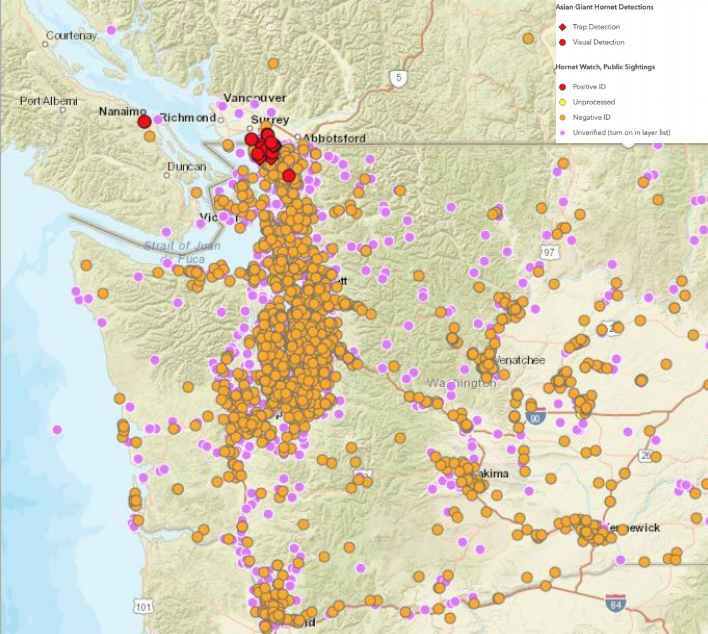
\includegraphics[width=7cm,height=7cm]{./pictures/dist0.png}
		\caption{ Asian Giant Hornet Detections\cite{website}}\label{nt}
	\end{minipage}
	\begin{minipage}{8cm}
		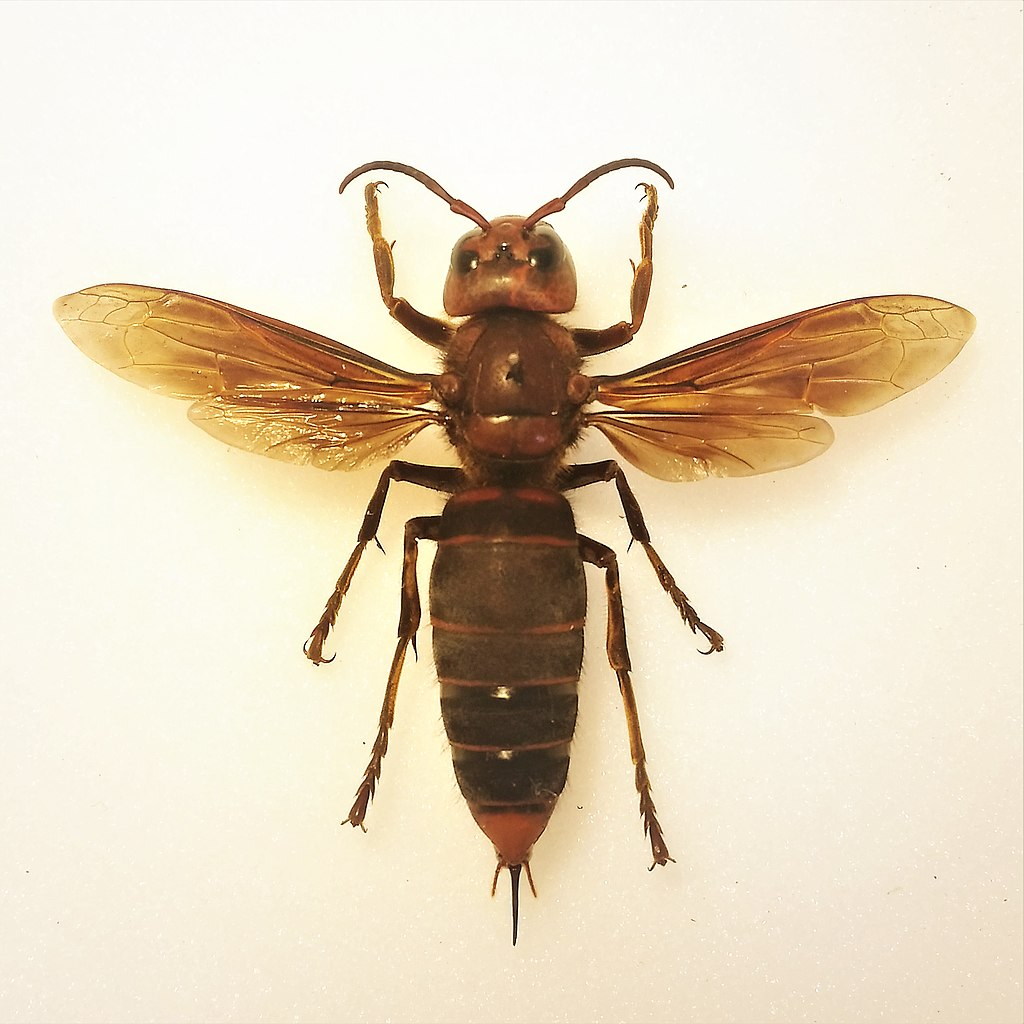
\includegraphics[width=7cm,height=7cm]{./pictures/wikiintro.jpg}
		\caption{\emph{Vespa mandarinia}\cite{wiki}}\label{nt}
	\end{minipage}
	
\end{figure}

\textbf{Name}
\begin{itemize}
	\item Common name:  Asian giant hornet, sparrow wasp,murder hornet
	\item Scientific name: Vespa mandarinia Smith, 1852
\end{itemize}

\textbf{Range of Activity }

Usually to find food, the Asian giant hornet goes only 0.5 to 1.25 miles (1-2 kilometers) away from the nest (and never more than 5 miles (8 kilometers)) .

\textbf{Life Period}

 Like other social wasps, Asian giant hornets are an annual species that build new nests every year. When winter arrives, the current seasons' nests die out and the only individuals that survive are overwintering queens. When overwintering queens emerge in the spring, they seek out protected areas in the ground to begin building a nests.
\quad\\
 
\textbf{Comparision with Other Species}

While Asian giant hornets do not occur in eastern North America, there are a number of other large wasps that may be confused for them.Here introduce some species alike and there distinctions.
\begin{table}  
	\caption{Similar Species}  
	\begin{center}  
		\begin{tabular}{|p{5cm}|p{7cm}| p{5cm}|}  
			\hline  
			Species & Similarity & Dinstinguish  \\ \hline  
			Asian Giant Hornet& around 1.5 inches,yellow head,black belly,live on the ground or lower than 6 foots&\\ \hline  
			VespaCabro & size,shape,color are simlilar &small differences on face and chest,live higher than 6 foots \\  
			\hline 
			VespulaSquamosa & only the queen may be confused in spring  &much smaller in size \\  
			\hline  
			cicada killers & simliar size  &no yellow in head and belly \\  
			\hline
			Dolichovespula Maculata &  &small size,in the color of black and white,live on the tree or reef\\  
			\hline
		\end{tabular}  
	\end{center}  
\end{table}




\subsection{Our work}
\begin{itemize}
	\item Firstly,we try to predict the spread of hornet ,but just find that the spread is not regulated.
	\item Secondly,from all the information WSDA recieved ,several confirmed sightings of the pest have occurred in neighboring Washington State, as well as a multitude of mistaken sightings.So we construct a model to distinguish whether or not the observed object in one sighting record is Asian Giant Hornet.
	\item Then,we use this model into unverified records to figure out the identity of the object.
	\item And we find methods to update the model as new data comes in.
	\item Finally, we use the result to verify that the hornet in Washington State has been readicated.
\end{itemize}


\section{Assumptions and Notations}

\subsection{Assumptions}
To simplify our model and eliminate the complexity, we make the following main assumptions in this literature. All assumptions will be re-emphasized once they are used in the construction of our model:
\begin{enumerate}[\bfseries 1.]
	\item e assume that the data given by official can fully solve the problem of the topic and do not need to obtain additional data as auxiliary information.
	\item Assumption2.
	\item Assumption3.
\end{enumerate}
\subsection{Notations}
In this work, we use the nomenclature in  \textbf{Table \ref{Ntt}} in the model construction. Other nonefrequent-used symbols will be introduced once they are used.

\begin{enumerate}[\bf 1.]
	\item work1.
	\item work2.
	\item work3.
	\item work4.
\end{enumerate}
\begin{table}[H]
	\begin{center}
		\caption{Notations}
		\begin{tabular}{cl}
			\toprule
			\multicolumn{1}{m{3cm}}{\centering Symbol}
			&\multicolumn{1}{m{8cm}}{\centering Definition}\\
			\midrule
			$I$&The Intensity of the Heat Source\\
			$k$&The Material's Conductivity\\
			$h$&The Heat Transfer Coefficient\\
			$c$&The Heat Capacity of Water (=4200 J/(kg$\cdot^\circ$C))\\
			$\rho$&The Density of Water (=10$^3$ kg/m$^3$)\\
			\bottomrule
		\end{tabular}\label{Ntt}
	\end{center}
\end{table}







\newpage
\section{Problem 1:The Spread of Hornet}
As we want to figure out the regulation of the pread of hornets,we divide the process into two parts:the first is \textbf{Data preprocessing}.Firstly,we draw related pictures and tables to get more intuition.Then we process data for further analysis.The second is to test and try to find out the regularity of the pread of hornet by \textbf{Hypothesis testing theory}.

\subsection{Data Preprocessing}
Firstly we want to know about the basic information of these sighting records
\begin{table}[H]
	\caption{Basic Information of records}  
	\large
	\begin{center}  
		\begin{tabular}{|p{7cm}|p{7cm}|}  
			\hline  
			Positive number & 14  \\ \hline  
			Negative number& 2096\\ \hline  
			Unverified number &2342 \\  
			\hline 
			Unprocessed & 15 \\  
			\hline  
			Date range &2018-06-19   to   2020-08-01 \\  
			\hline
		    Latitude range & 45.4886  --   49.5480\\  
			\hline
			Longitude range & -124.6650   --  116.8736\\  
			\hline
		\end{tabular}  
	\end{center}  
\end{table}

According to the table above,we decide to choose process data in these way:
\begin{itemize}
	\item Select positive ID and unverified sample to anlysis.That's because the sample of Positive ID is too small and  random.
	\item Use the average position of each month's sighting site as the center of hornet, and search the tend of the species by the change of center point.
	\item Use the data after March,2019.For it's when the first confirmed sighting appeared.
\end{itemize}

\begin{figure}[H]
	\centering
	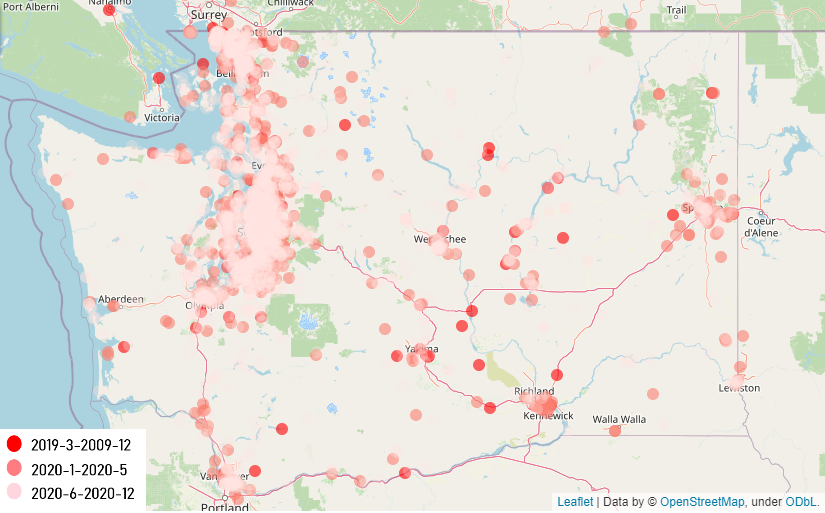
\includegraphics[width=14cm,height=7cm]{./pictures/distribute1.png}
	\caption{sighting sites}\label{nt}
\end{figure}

\begin{figure}[H]
	\small
	\centering
	\begin{minipage}{8cm}
		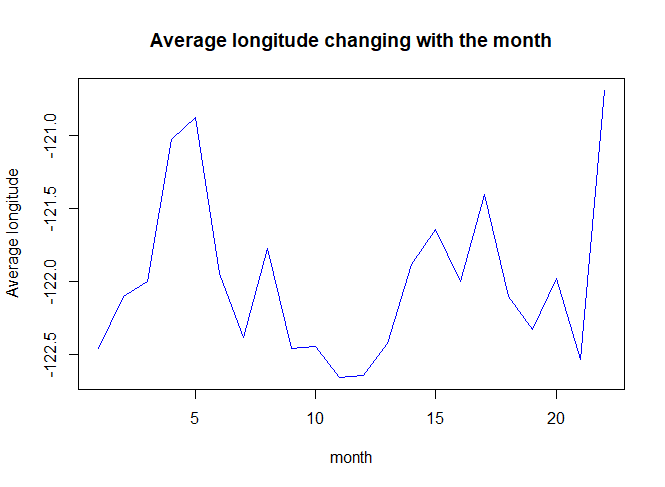
\includegraphics[width=8cm,height=7cm]{./pictures/longtitude.png}
		\label{nt}
	\end{minipage}
	\begin{minipage}{8cm}
		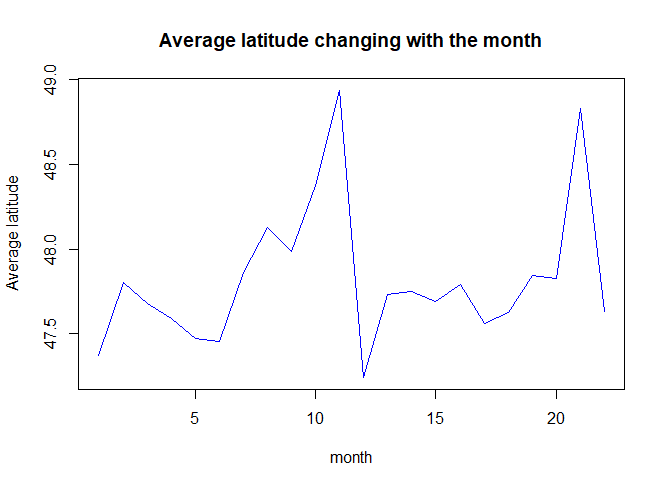
\includegraphics[width=8cm,height=7cm]{./pictures/latitude.png}
		\label{nt}
	\end{minipage}
	\caption{The change of center point}
\end{figure}
From the pictures above ,we find out that the movement of hornet is quite random,so we need to use some statistic methods to approve that.

\subsection{Hypothesis Testing}
\subsubsection{Model}
We want to test whether the center points of hornet are related by time or the route of the colony has some regulation.So we hypothesis that:
\begin{equation*}
H0:\textbf{These center points are independent }\leftrightarrow H1:\textbf{These center points are not independent}
\end{equation*}

And for it's two dimension data,we test the regulation in longitude and latitude apparently.

As we use $\rho_i$ to represent the k-order lag correlation coefficient of the sample's longtitude.The  hypothesis can be writen as:
\begin{equation*}
H0:\rho_1^2=\rho_2^2=...\rho_h^2 \leftrightarrow H1:\exists k,s.t. \rho_k^2\neq 0
\end{equation*}
And choose pivot quantity
\begin{equation*}
Q=n(n+1)\sum_{k=1}^h \frac{\rho_k^2}{n-k},\qquad ,h:degree \,of\, randomness
\end{equation*}
For $Q\sim \chi^2(h)$,as significance level is $alpha$,the rejection region is $Q> \chi^2_{\alpha-1}(h)$.

In the same way,we test the randomness of the latitude data by using latitude information to calculate $\bar\rho_i\,and\,\bar{Q}$.

\subsubsection{Conclusion}
According to calculating result,neither $Q$ and $\bar{Q}$ doesn't fall in the  the rejection region even in the significance level of 0.5 (P-value are above 0.5 in whatever the randomness is ).\textbf{That means we can't say the spread of hornet can be predicted even the accuracy is 0.5}

\section{Problem 2:Classification Model}
\subsection{Model Introduction}
From all the records we get information in quite a lot of forms including \textbf{word,image,video and so on}.
\begin{itemize}
	\item \textbf{Video}:video of the recorded object,including video after capture the insect,surveillance video contains the insect ,video of outdoor observation and so on.
	\item \textbf{Image}:image with the recorded insect held on hand,captured by bottl,on a web,in flowers and so on.
	\item \textbf{Word}:notes recorded by the observer;comments replied by the officer。
	\item \textbf{Other information}:longitude and latitude of the sighting site and the date.
	\item \textbf{Label Status}:whether or not the object is Asian Giant Hornet ,including unverified.
\end{itemize}

So,we choose \textbf{Multimodal machine learning} to classify the records.
That means we use all the given information to construct the classification model.

\quad \\
Another key porblem of this issue is :the positive sample is too small (14 compared with the negative sample number:2096).So the \textbf{sample imbalance} is great.We use \textbf{sample augmentation,focal loss ,oversampling} to deal with this problem.

A more detailed explaination of the model can be seen in the picture below:
\begin{figure}[H]
	\centering
	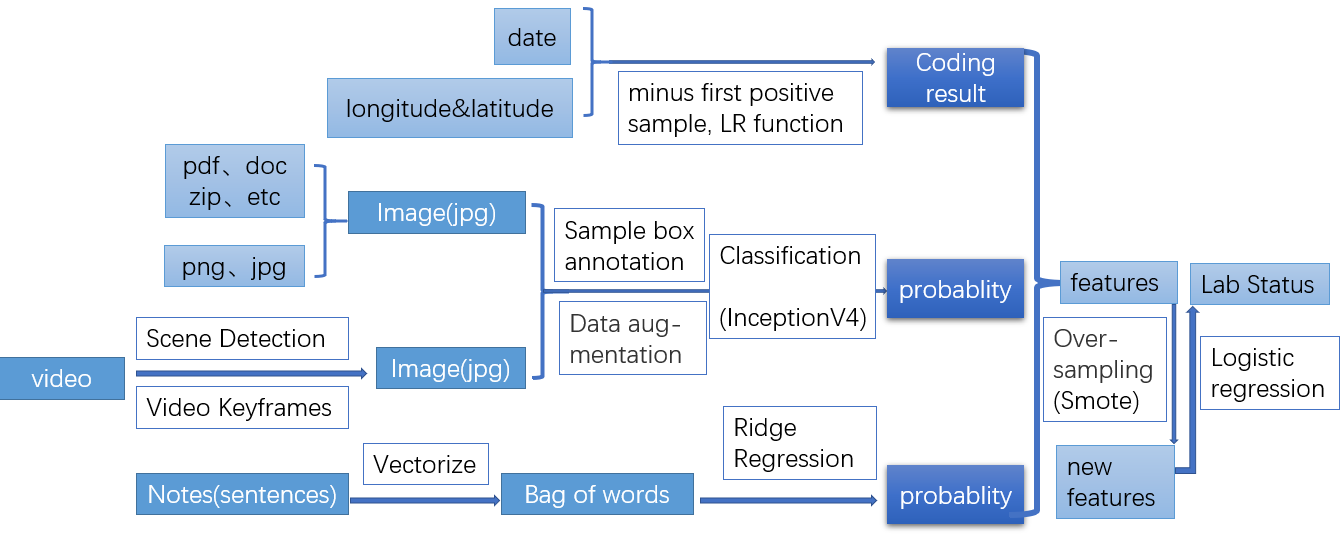
\includegraphics[width=18cm,height=8cm]{./pictures/problem2.png}
	\caption{Multimodal Classification Model}\label{nt}
\end{figure}


\subsection{Date,Longitude and Latitude Coding}
To deal with these three index,we do two steps:
\begin{enumerate}
	\item choose the first positive sample as reference(for date we counts the days between two samples) to eminate the influence of magnitude.
	\item \textbf{ LR function} for date:$f(x)=\left\{\begin{matrix}
	\frac{1}{x} & |x|>1 \\ 
	1 & |x|\leq 1
	\end{matrix}\right.$ to limit the number.
	\item \textbf{ LR function} for longitude and latitude:$g(x)=x$,for the numbers are all less than 1.
\end{enumerate} 

\subsection{Video Processing}
In the given reports there are 92 vedio.Some videos almost keep quiet and can get quite clear image of the object,while others may contains great movement and can not recognize things clearly.In order to use all these information completely, we use \textbf{Scene Detection}to recognize \textbf{Scene Boundaries} and get\textbf{Video Keyframes} from video and porcess them with images together.

\subsubsection{Scene Detection}
Video scene detection algorithms generally use the degree of similarity difference between frames to measure, if the video frame is greater than a certain threshold, it is considered a new scene, otherwise it is not a new scene.

To do this there are mainly two ways:
\begin{itemize}
	\item \textbf{scikit-video}\cite{scikitvideo}:it uses the similarity between color and fringe to detect.
	\item \textbf{ffmpeg}\cite{ffmpeg}:it chooses the frames considering the compression degree
\end{itemize}
Compared these two methods we use ffmpeg for it's quicker and moere efficient.

\subsubsection{Video Keyframes}
Video Keyframes are frames used for Video compression and Video codec and contain complete information. Other non-key frames will be compressed by the difference between them. Video frames can be divided into three types:
\begin{itemize}
	\item \textbf{I} :frame represents the key frame and is the most complete frame. Generally, I frame is selected for the video cover.
	\item \textbf{P} :frame single prediction frame, using the previous I frame or P frame, using motion prediction method for interframe prediction coding.
	\item \textbf{B} :frame bidirectional prediction frame, using bidirectional frame prediction coding.
\end{itemize}

And we firstly use \textbf{ffprobe} to get IBP frames,and than combine them to construct jpg image.


\subsection{Image Processing}
After combine the image provided and the image produced from the video,we cope with them in two ways:
\begin{enumerate}
	\item \textbf{Sample box annotation} 
	\item \textbf{Data augmentation}
\end{enumerate}
to make the information for efficient thus improve classification's accuracy.


\subsubsection{Sample Box Annotation}
In many pictures,the insect is hidden in the environment such as flowers and woods and the size of the insect is small.

So it's hard to distinguish the insect through these pictures.To deal with these we try to annotate the sample box.For the amount of pictures is large,we do this by  \textbf{YoloV5}\cite{Yolo},an auto-annotate algorithm:
\begin{itemize}
	\item  First we annotate the sample box by hand to get 750 picture as trian data.
	\item  Then we use YoloV5 to deal with more than 2000 pictures.
\end{itemize}
The annotation result is pretty good as we can see in the picture below.

And as we can see in \ref{box},the sizes of sample boxes are not uniform,so it's neccessary to do \textbf{Sample Box Annotation} to extract information correcetly.

\begin{figure}[H]
	\small
	\centering
	\begin{minipage}{5cm}
		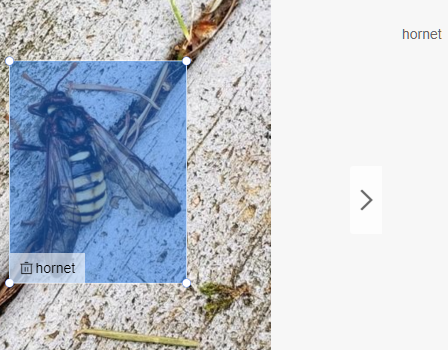
\includegraphics[width=5cm,height=5cm]{./pictures/hand1.png}
		\label{nt}
	\end{minipage}
	\begin{minipage}{5cm}
		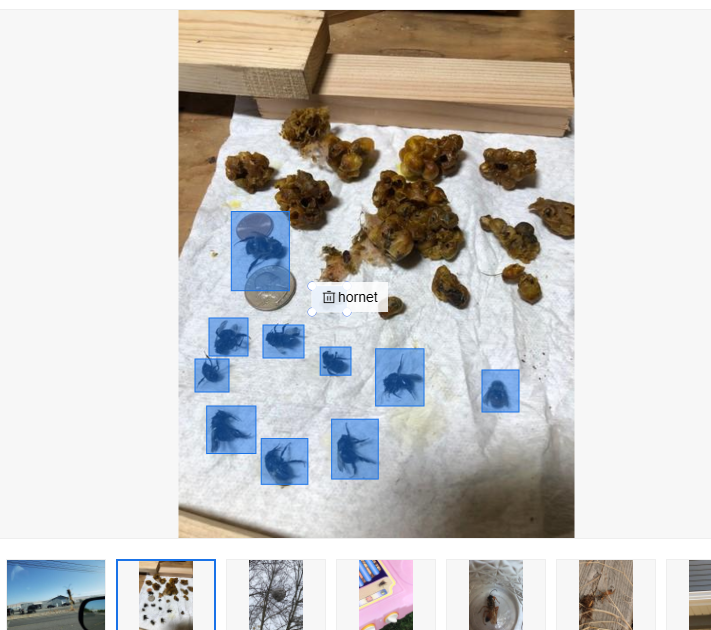
\includegraphics[width=5cm,height=5cm]{./pictures/head2.png}
		\label{nt}
	\end{minipage}
	\begin{minipage}{5cm}
		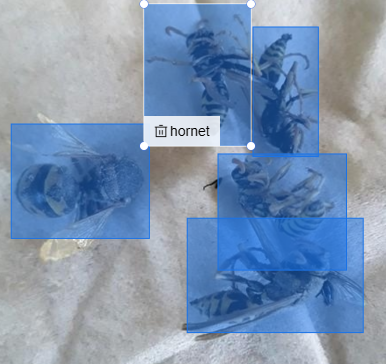
\includegraphics[width=5cm,height=5cm]{./pictures/head3.png}
		\label{nt}
	\end{minipage}
	\caption{Sample box annotation by hand}
\end{figure}
\begin{figure}[H]
	\small
	\centering
	\begin{minipage}{7cm}
		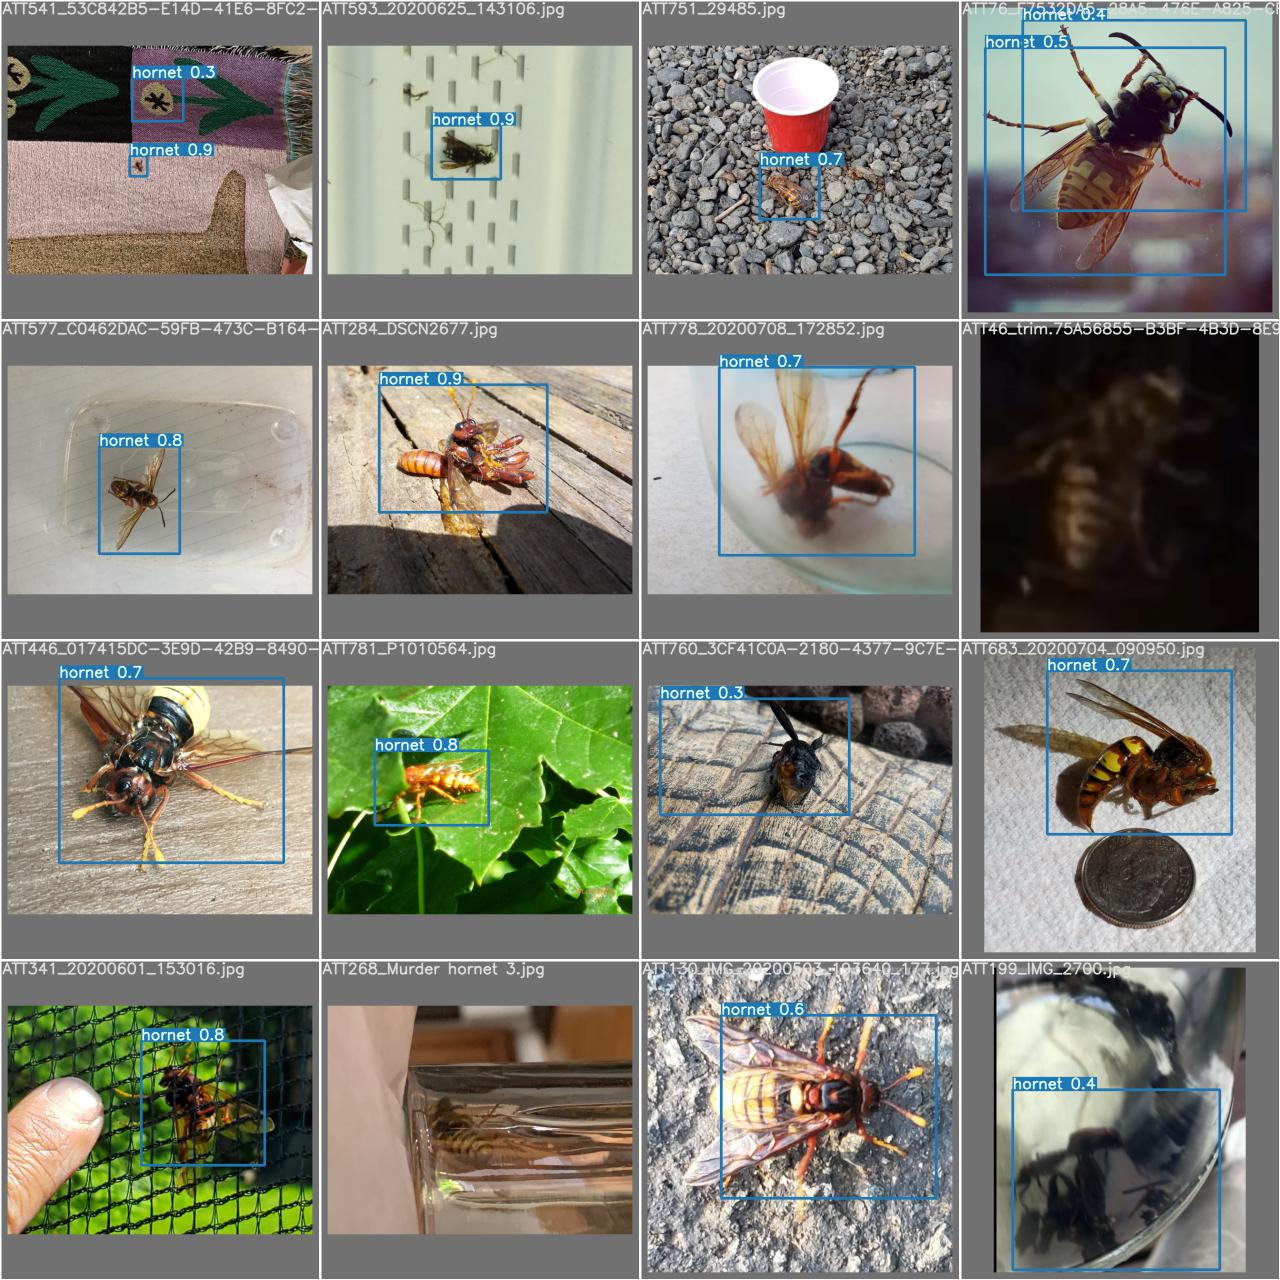
\includegraphics[width=7cm,height=6cm]{./pictures/machine1.png}
		\caption{Sample box annotation by yolo}\label{nt}
	\end{minipage}
	\begin{minipage}{7cm}
		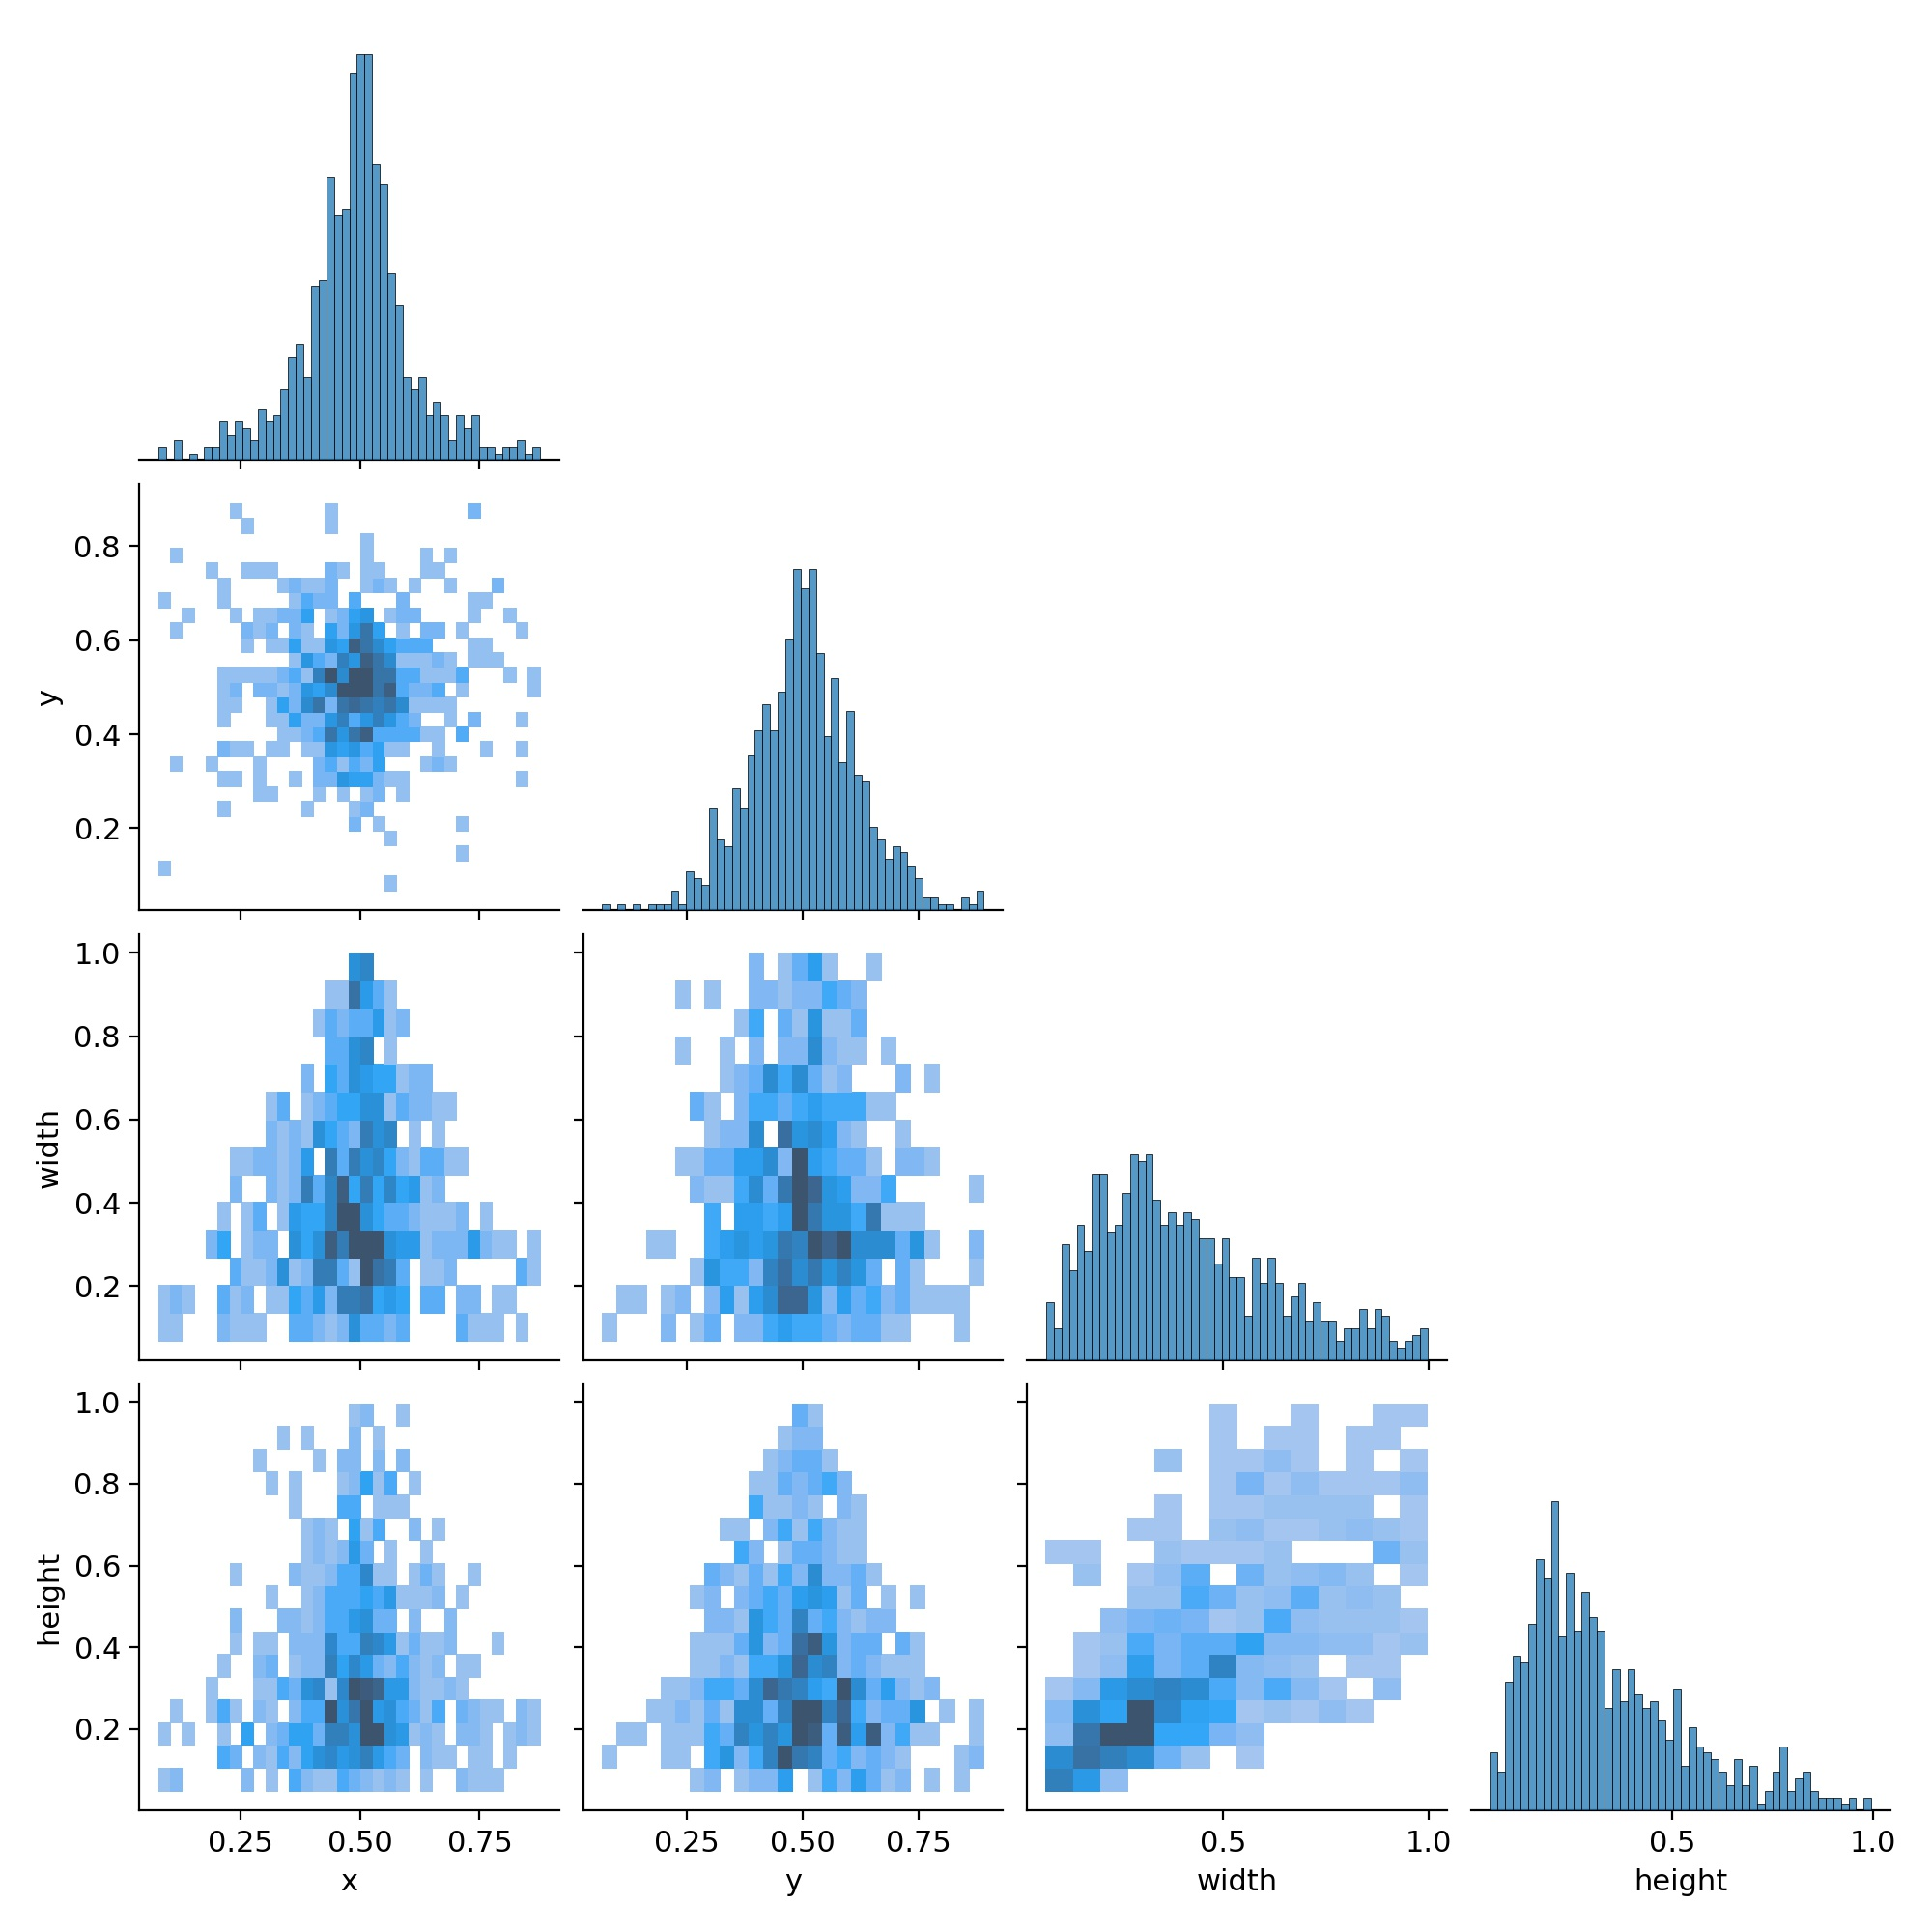
\includegraphics[width=7cm,height=6cm]{./pictures/picture_correlogram.png}
		\caption{the size and position sample box\protect\footnotemark[1]}
		\label{box}
	\end{minipage}
\end{figure}
\footnotetext[1]{x,y reprsent middle point of the sample box,width and hight describe the shape. }

\subsubsection{Data Augmentation}
For the number of positive sample is too small, we use \textbf{data augmentation} to create more pictures from one positive sample through photo change.Thus we can get more information about how Asian Giant Hornet looks like.

As \ref{box} shows,the size and shape of the sample box is not regular(The center of the sample frame is normally distributed and the height and width are skewed) ,so we choose to do the change randomly,that's to say the angle we rotate or the size we cut and other parameter are choosen randomly,so we can get more useful information.

More detailed operation can be seen in the table\ref{augm},and a result can be seen in the picture\ref{augres}.

\begin{table}[H]
	\caption{Data augmentation operation}  \label{augm}
	\small
	\begin{center}  
		\begin{tabular}{|p{2cm}|p{14cm}|}  
			\hline  
			Operation &   python code\footnotemark[2]\\ \hline  
			Flip& RandomHorizontalFlip(),
			RandomVerticalFlip()\\ \hline  
			Rotation &RandomRotation(180, expand=True),
			RandomRotation(180, expand=False),\\  
			\hline 
			Affine& andomAffine(180, (0.3, 0.3), (0.4, 1), 3) \\  
			\hline  
			   Crop&RandomResizedCrop(size),
			   transforms.RandomCrop(size, pad\_if\_needed=True),
			   transforms.CenterCrop(size),
			   transforms.RandomPerspective(distortion\_scale=0.3) \\  
			\hline
			 Color &  transforms.RandomGrayscale(0.2),
			 transforms.GaussianBlur(9),
			 transforms.ColorJitter(0.8, 0.8, 0.8, 0.4)\\  
			\hline
	
		\end{tabular}  
	\end{center}  
\end{table}
\footnotetext[2]{Python code using torchvision.transforms package. }


\begin{figure}[H]
	\small
	\centering
	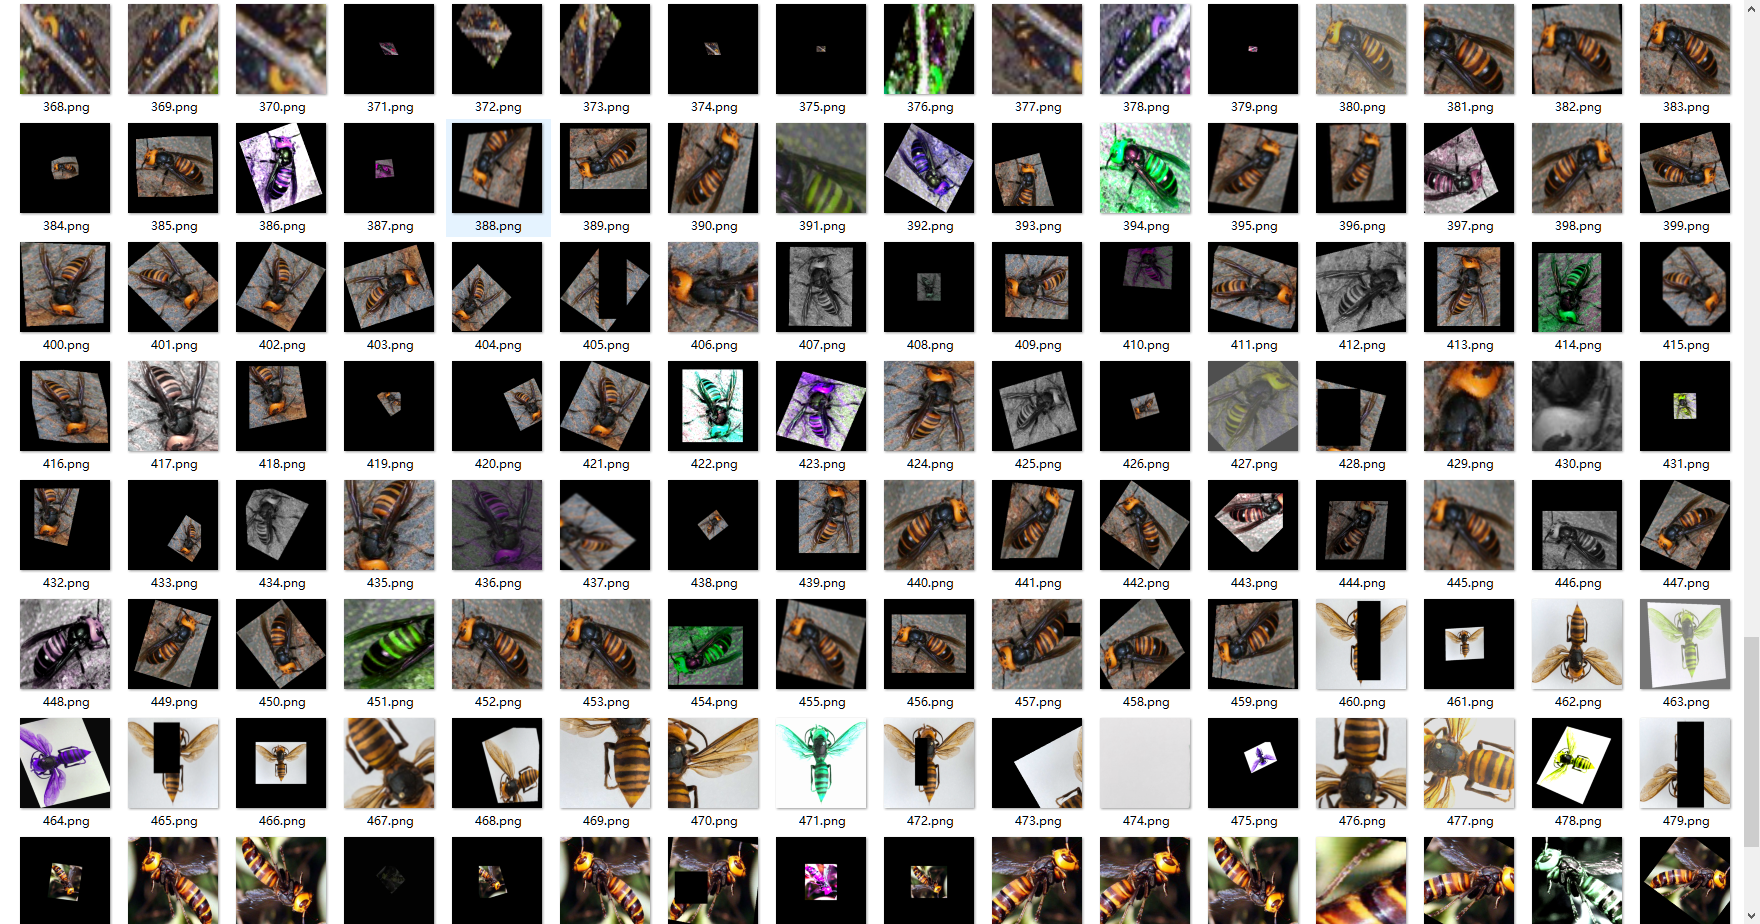
\includegraphics[width=14cm,height=6cm]{./pictures/angres.png}
	\caption{Data augmentation result}\label{augres}

\end{figure}


\subsection{Image Characteristics Extraction}
After we process all the image and video, we get dozens of pictures.Then we need to extract features from these samples for further classification.

To do this,we choose a \textbf{CNN model} by GoogLeNet:\textbf{Inception V4}. For it's much quicker than Resnet and other picture classification networks.

\subsubsection{Focal Loss}
\textbf{Thro}


\subsection{Language Processing}
In the given infomation,there are notes with each record,to deal with the words we need to code them first.We use \textbf{N-grams} to \textbf{vectorize} the sentence.This takes two steps:
\begin{enumerate}
	\item take adjacent words to construct combinations.
	\item represent the combinations with their frequency in whole sample.
\end{enumerate}
Through then we change a sentence into a string of numbers.



\section{Targets and Action}
\section{Senitivity Analysis}\label{condition}
\section{ Strengths and Weaknesses}
\subsection{Strengths}
\begin{itemize}
	\item Strength1.
	\item Strength2.
	\item Strength3.
\end{itemize}
\subsection{Weaknesses}
\begin{itemize}
	\item Weakness1.
	\item Weakness2.
\end{itemize}
\section{conclusion}
Different methods may show different ranks of effect according to the users' demand, the conditions
outside the bathtub and of the bathtub, and so on. However, according to our research in Section
\ref{condition}, these recommended methods are still useful under various conditions, if the details
(e.g. the temperature and the time of period) are properly adjusted. So the users can choose and
adjust the bath strategy based on the rules below:

\paragraph{Rule I}
\emph{High temperature and large flux can make the water attach the optimum temperature earlier,
	meanwhile it may cause uneven temperature and waste of water.}
\paragraph{Rule II}
\emph{Evenness comes from continuous inflow with appropriate temperature, a little higher than the
	optimum temperature in usual.}
\paragraph{Rule III}
\emph{The best strategy to have an excellent bath is to heat up the water before it cool down.}

\clearpage
\section*{Memo}\addcontentsline{toc}{section}{Memo}
	\begin{flushleft}
		Dear users:
	\end{flushleft}
	
	Thank you very much for choosing our bathtubs. Each piece of your support is our valuable treasure
	which can encourage us to develop better bathtubs.We express our sincere thanks to you and your
	family!
	For this kind of bathtub, we have some suggestions for you:
	\begin{enumerate}[\bf 1.]
		\item You don't have to worry about the full-water condition, because when the bathtub is full
		of water, the overflow drain can drain out the excess water.
		\item With the consideration that you will have your special demands on the bath water, we give
		you some suggestion through so that you can choose what you prefer
		(or just freestyle you bath).
		
	\end{enumerate}
\clearpage
\begin{thebibliography}{99}
	\addcontentsline{toc}{section}{References}  %引用部分标题("Refenrence")的重命名
	\bibitem{fb}Facebook.Asian Giant Hornet Watch.https://www.facebook.com/groups/hornets.
	\bibitem{website}Washington State Department of Agriculture. 2020 Asian Giant Hornet Public 
	Dashboard. https://agr.wa.gov/departments/insects-pests-and-weeds/insects/hornets/data.
	\bibitem{wiki}Wikipedia.Asian Giant Hornet. https://en.wikipedia.org/wiki/Asian\_giant\_hornet.
	\bibitem{scikitvideo}Scikit-Video .https://github.com/scikit-video/scikit-video/blob/master/skvideo/measure/scene.py.
	\bibitem{ffmpeg}ffmpeg . https://ffmpeg.org/ffmpeg-filters.html\#select\_002c-aselect.
	\bibitem{Yolo}YoloV5 . https://github.com/topics/yolov5
	\bibitem{10}Lu J.A., Shang A., Xie J., Gu P., MATLAB-Solution of Partial Differential Equations (in
	Chinese). \emph{Wuhan University Press}, 2001.

\end{thebibliography}

\clearpage

\section*{Appendices}\addcontentsline{toc}{section}{Appendices}
	\noindent Appendix1:
	%下面的是配置是可以写中文注释的python环境:
	%\usepackage{listings}
	%\usepackage{color}
	\definecolor{dkgreen}{rgb}{0,0.6,0}
	\definecolor{gray}{rgb}{0.5,0.5,0.5}
	\definecolor{mauve}{rgb}{0.58,0,0.82}
	\lstset{	frame=shadowbox,                           % shadowbox framed
		rulesepcolor= \color{gray},%框的颜色
		language=Python,
		aboveskip=3mm,
		belowskip=3mm,
		showstringspaces=false,
		columns=flexible,
		basicstyle={\small\ttfamily},
		numbers=left,%设置行号位置none不显示行号
		%numberstyle=\tiny\courier, %设置行号大小  
		numberstyle=\tiny\color{gray},
		keywordstyle=\color{blue},
		commentstyle=\color{dkgreen},
		stringstyle=\color{mauve},
		breaklines=true,
		breakatwhitespace=true,
		escapeinside=``,%逃逸字符(1左面的键),用于显示中文例如在代码中`中文...`
		tabsize=4,
		extendedchars=false %解决代码跨页时,章节标题,页眉等汉字不显示的问题  
	}
	\begin{lstlisting}
	# Scene Detection
	ffmpeg -i “video name” -filter:v "select='gt(scene,0.1)',showinfo" -f null - 2>&1
	ffmpeg -i 666051400.mp4 -filter:v "select='gt(scene,0.1)',showinfo" -f null - 2>&1
	#ues ffprobe get IPB time:
	ffprobe -i 666051400.mp4 -v quiet -select_streams v -show_entries frame=pkt_pts_time,pict_type
	#transform IPB to jpg:
	ffmpeg -i 666051400.mp4 -vf "select=eq(pict_type\,I)"  -vsync vfr -qscale:v 2 -f image2 ./%08d.jpg
	\end{lstlisting}
	
	

%%%%%%%%%%%%%%%%%%%%%%%%%%%%%%
\end{document}
